\documentclass[a4paper]{article}

%% Language and font encodings
\usepackage[english]{babel}
\usepackage[utf8x]{inputenc}
\usepackage[T1]{fontenc}

%% Sets page size and margins
\usepackage[a4paper,top=3cm,bottom=2cm,left=2.7cm,right=2.7cm,marginparwidth=1.75cm]{geometry}

%% Useful packages
\usepackage{amsmath}
\usepackage{amsfonts}
\usepackage{bm}
\usepackage{graphicx}
\usepackage[colorinlistoftodos]{todonotes}
\usepackage[colorlinks=true, all colors=blue]{hyperref} %referenze linkate
\usepackage{booktabs}
\usepackage{siunitx}  %notaz. espon. con \num{} e unità di misura in SI con \si{}
\usepackage{xcolor}
\usepackage{colortbl}
\usepackage{bm}
\usepackage{caption} 
\usepackage{indentfirst}
\usepackage{physics} 
\usepackage{rotating}
\usepackage{tabularx}
\usepackage{url}
\usepackage{pst-plot}
\usepackage{comment} %per usare l'ambiente {comment}
\usepackage{float} 
\usepackage{subfig}
\usepackage[americanvoltages]{circuitikz} %per disegnare circuiti
\usepackage{tikz}
\usepackage{mathtools} %per allineare su più linee in ambiente {align} o {align*}
\usepackage{cancel}
\usepackage{listings}
\renewcommand{\CancelColor}{\color{lightgray}}
%\setlength{\parindent}{0cm}


%%%%%%%%%% HEADERS AND FOOTERS %%%%%%%%%%%%
\newcommand{\theexercise}{Ex. 2}
\newcommand{\thedate}{October 20, 2020}
\usepackage{fancyhdr}

\pagestyle{fancy}
\fancyhf{}
\lhead{Giorgio Palermo}
\rhead{\thedate}
\lfoot{Quantum Information 20/21}
\cfoot{\theexercise}
\rfoot{Page \thepage}

%%%%%%%%%% CODE LISTING %%%%%%%%%%%
%New colors 
\definecolor{codegreen}{HTML}{92c42a}
\definecolor{codegray}{rgb}{0.5,0.5,0.5}
\definecolor{codepurple}{HTML}{f92472}
\definecolor{codeblue}{HTML}{67d8ef}
\definecolor{codeyellow}{HTML}{e68f29}%{e4ab24}
\definecolor{codemagenta}{HTML}{f92472}
\definecolor{backcolour}{rgb}{0.95,0.95,0.92}


%Code listing style named "mystyle"
\lstdefinestyle{mystyle}{
  language={[03]Fortran},
  backgroundcolor=\color{backcolour},   commentstyle=\color{codegray},
  keywordstyle=\color{codemagenta},
  numberstyle=\tiny\color{codegray},
  stringstyle=\color{codeyellow},
  basicstyle=\ttfamily\footnotesize,
  breakatwhitespace=false,         
  breaklines=true,                 
  captionpos=b,                    
  keepspaces=true,                 
  numbers=left,                    
  numbersep=5pt,                  
  showspaces=false,                
  showstringspaces=false,
  showtabs=false,                  
  tabsize=2
}
%"mystyle" code listing set
\lstset{style=mystyle}


\graphicspath{{Figure/}}
\captionsetup{format=hang,labelfont={sf,bf},font=small}
\captionsetup{tableposition=top,figureposition=bottom,font=small}
\captionsetup[table]{skip=8pt}







\begin{document}
\hypersetup{linkcolor = black}
\hypersetup{linkcolor = blue}
\thispagestyle{plain}
\begin{center}
    \textbf{MASTER'S DEGREE IN PHYSICS}
    
    Academic Year 2020-2021
    
    \medskip
    \textbf{QUANTUM INFORMATION}
\end{center}

\vspace{0.0cm}
Student: Giorgio Palermo

Student ID: 1238258

Date: \thedate
\begin{center}
\textbf{EXERCISE 2}
\medskip
\end{center}
\noindent
\textit{In this report I will review my solution to EX2, which is about the definition of new types, functions, subroutines and interfaces.}

\section*{Theory}
I based my solution of the proposed exercise on the definition of the \lstinline{type}, \lstinline{function}, \lstinline{subroutine} and \lstinline{interface} constructs reviewed in class.

\section*{Code Development}
The basic brick of this program is the \lstinline{dmatrix} type, which I defined as a new type containing a \lstinline{double complex} matrix and some of its properties: shape, track and determinant.
\begin{lstlisting}
type dmatrix
    integer, dimension(2) :: N = (/ 0,0 /)
    double complex, dimension(:,:), allocatable :: elem
    double complex :: Trace
    double complex :: Det
end type dmatrix
\end{lstlisting}

The \lstinline{InitUni} function is a \lstinline{type(dmatrix)} function that calls the \lstinline{clarnv} LAPACK subroutine to fill the matrix (\lstinline{dmatrix%elem}) with random complex numbers.
Since \lstinline{clarnv} only works on scalar or vectors, I implemented a cycle to fill the matrix; I chose to loop over columns because this is the fastest algorithm since the matrix is stored column-wise.

\noindent I decided that in my program the shape of a \lstinline{dmatrix} has to be defined separately before the call to the initialization function, therefore I put a check at the beginning of it to verify that both dimensions are defined and positive.
\begin{lstlisting}
function InitUni(dmat) 
    ! Initializes a (m,n) complex matrix with 
    ! real and imaginary part taken from [0,1]
    ! uniform distributions
    implicit none
    type(dmatrix), intent(in) :: dmat
    type(dmatrix) :: InitUni
    integer :: jj,sd=4
    integer, dimension(:), allocatable :: seed
    double complex, dimension(dmat%N(1),1) :: X

    if(dmat%N(1)<1 .or. dmat%N(2)<1) then
        ! Check for positive matrix shape
        print*, "*** ERROR in InitUni: matrix shape not defined"
        print*, "Program terminated"
        stop
    else
        call random_seed(size = sd)
        allocate(seed(sd))
        call random_seed(get=seed)
        do jj=1,dmat%N(2)
            ! '1' stands for uniform
            call clarnv(1, seed, 2*dmat%N(1), dmat%elem(:,jj) )
        end do
        InitUni = dmat
        return
    end if
end function InitUni
\end{lstlisting}

The \lstinline{Tr} subroutine computes the trace summing over diagonal elements of a \lstinline{dmatrix%elem} matrix given as input.
\begin{lstlisting}
subroutine Tr(dmat)
    ! Computes the trace and assigns it
    ! to the "Trace" field of the input object
    ! of type dmatrix
    type(dmatrix) :: dmat
    integer ::ii
    if(dmat%N(1)==dmat%N(2) .and. dmat%N(1)>0 .and. dmat%N(2) >0) then
        do ii=1,dmat%N(1)
            dmat%Trace=dmat%Trace +dmat%elem(ii,ii)
        end do
        return
    else
        print*, "*** ERROR in Tr: matrix dimensions must be positive and equal"
        return
    end if
end subroutine Tr
\end{lstlisting}

\lstinline{Adj} is a \lstinline{type(dmatrix)} function which aim is to compute the transposed conjugate of a \lstinline{type(dmatrix)} input.
To do this it copies an input \lstinline{dmatrix} type element into a local new variable and computes the adjoint using the intrinsic elemental function \lstinline{conjg()}; the transposition is then performed using the intrinsic \lstinline{transpose()} function.
\begin{lstlisting}
function Adj(dmat)
    ! computes the adjoint and passes it
    ! as output
    type(dmatrix),intent(in) :: dmat
    type(dmatrix) ::Adj
    Adj%Trace=conjg(dmat%Trace)
    Adj%Det=conjg(dmat%Det)
    Adj%N=(/ dmat%N(2), dmat%N(1) /)
    allocate(Adj%elem(Adj%N(1),Adj%N(2)))
    Adj%elem=dmat%elem
    Adj%elem=conjg(Adj%elem)
    Adj%elem=transpose(Adj%elem)
    return
end function Adj
\end{lstlisting}

\noindent I assigned the \lstinline{Adj} and the \lstinline{InitUni} functions to two interface operators: \lstinline{.Adj.} and \lstinline{.Init.}.
\begin{lstlisting}
interface operator (.Adj.)
        module procedure Adj
end interface 

interface operator (.Init.)
    module procedure InitUni
end interface
\end{lstlisting}

All these functions, subroutines and interfaces are defined inside a module.

\section*{Results}
All the functions and subroutines are tested in a simple program, \lstinline{DMatrixCODE}, which calls all the above mentioned functions and operators.
More specifically, it defines and initializes a new \lstinline{dmatrix} type variable, computes its trace and adjoint and writes both the matrix and its adjoint to file, using the subroutine \lstinline{MatToFile} which I implemented to do this job.
\begin{lstlisting}
program DMatrixCODE
    use stuff
    implicit none
    type(dmatrix) :: dmat, dmat1
    integer, dimension(2) ::shape = (/ 2, 2 /)

    write(*,'(A,/,A,/)') "","    *** DMatrixCODE.f03 - Complex matrix manipulation ***  "
    
    dmat%N=shape
    allocate(dmat%elem(dmat%N(1),dmat%N(2)))
    allocate(dmat1%elem(dmat%N(1),dmat%N(2)))
    print*, "Initializing matrix..."
    dmat = .init.dmat
    print*, "Computing Trace, Adjoint..."
    call Tr(dmat)
    dmat1 = .Adj.dmat
    print*, "Writing results to file..."
    call MatToFile(dmat,"matrix")
    call MatToFile(dmat1,"matrix_conj")
    
    deallocate(dmat%elem,dmat1%elem)
    write(*,'(/,A)') "    *** End of the program"
end program
\end{lstlisting}

\noindent Hereafter are reported two typical outputs for a randomly initiated $2\times2$ matrix and its adjoint.

\begin{figure}[h!]
\centering
\subfloat{    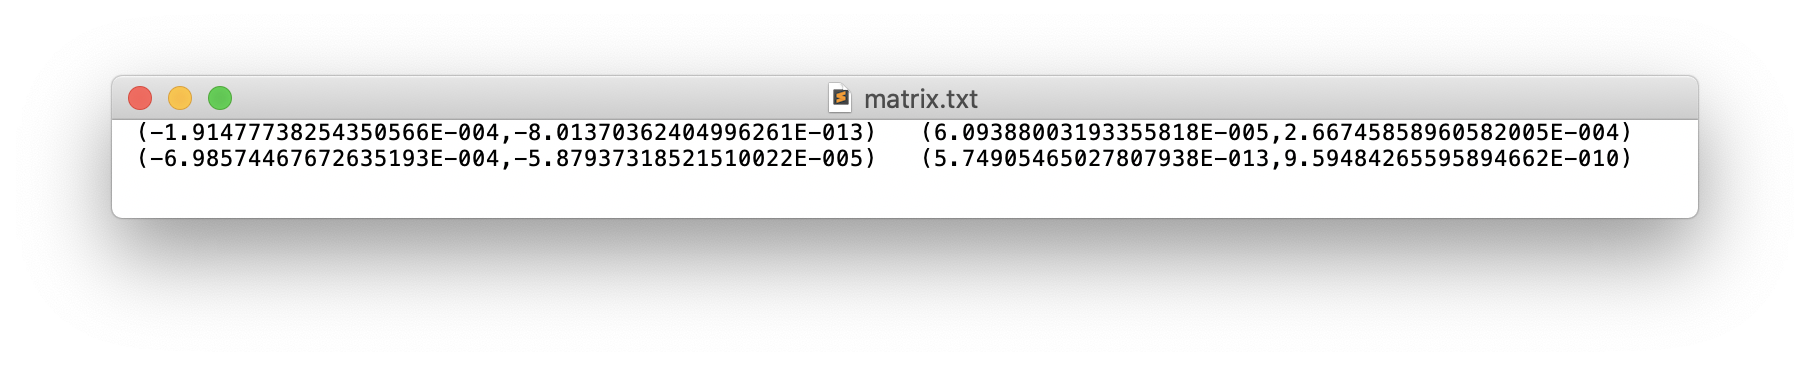
\includegraphics[width=\textwidth]{Mat.png} }

\vspace{-1cm}
\subfloat{    \includegraphics[width=\textwidth]{Mat_Conj.png}}
\vspace{-.5cm}
\caption{Output files examples}
\end{figure}
\section*{Self evaluation}
Writing this exercise I learned how to define new types, functions, subroutines and interface operators; I also learned to call external LAPACK functions and to compile the code including the linear algebra library.

\noindent I wonder if in \lstinline{Tr()} function is sufficient to check for the dimensions of the matrix to be positive or it would be recommendable to check if the memory for the \lstinline{dmatrix%elem} is already allocated, in order to avoid errors.





\end{document}
